\documentclass[10pt,aspectratio=169]{beamer}


%% foot adds a foot line to the frames including conference and date

%% logo adds the university logo on the left of the footer line

%% sectionintroframe adds an empty frame before each new section with the title of the section

%% nototalframenumber regularizes the display of the totalframenumber in the lower right
%% (e.g., '2' instead of '2/27')

%% nosectiontitlepage switches off the behaviour of inserting the titlepage every time a \section is called
% this makes it possible to use more than one section + thanks page and a ToC
% off by default


\usetheme[nototalframenumber,foot,logo,nosectiontitlepage]{_applmath}

%%Bibtex options
\usepackage[style=numeric, backend=bibtex,
giveninits=true]{biblatex}
\title[]{Self-Supervised Global-Local Segmentation for 3D Out-of-Distribution Detection}
\subtitle{\textsuperscript{1}University of Innsbruck\\ \textsuperscript{2}Medical University of Innsbruck}



\author[Angermann et al.]{Christoph Angermann \inst{1} \and Simon Göppel \inst{1} \and Markus Tiefenthaler \inst{2} \and Matthias Schwab \inst{2}}


%('short author' is the pdf-metadata Author)
%% If multiple authors are required and the font size is too large you
%% can overrule the font size of author and url by calling:
%\setbeamerfont{author}{size*={10pt}{10pt},series=\mdseries}
%\setbeamerfont{url}{size*={10pt}{10pt},series=\mdseries}
%\URL{}
%\subtitle{}

\footertext{Medical Out-of-Distribution Analysis Challenge 2022}
\date{}

\headerimage{4}

\usepackage{subcaption}
\usepackage{wrapfig}
\usepackage{tikz}
\usepackage{braket}
\usepackage{color}
\usepackage{mathtools}
\usepackage{amssymb}
\usepackage{amsthm}
\usepackage{amsmath}
\usepackage{amsfonts}
\usepackage{dsfont}
\usepackage{tikz-cd}
\usepackage{xcolor}
\usepackage{graphicx}



\newcommand\gauss[2]{1/(#2*sqrt(2*pi))*exp(-((x-#1)^2)/(2*#2^2))} 
\newcommand{\paren}[1]{\left(#1\right)}               % Klammern
\newcommand{\bparen}[1]{\left[#1\right]}               % eckige Klammern
\newcommand{\sparen}[1]{\left\{#1\right\}}		      % Mengenklammer
\newcommand{\sqparen}[1]{\left[#1\right]}             % eckige Klammern
\newcommand{\h}[1]{\left\langle#1\right\rangle}       % Skalarprodukt
\newcommand{\abs}[1]{\left|#1\right|}
\newcommand{\norm}[1]{\left\lVert#1\right\rVert} 
%\newcommand{\spn}[1]{\textup{span}\left\{#1\right\}} 

%Zahlbereiche
\newcommand{\C}{\mathds C}
\newcommand{\D}{\mathds D}
\newcommand{\N}{\mathds N}
\newcommand{\Q}{\mathds Q}
\newcommand{\R}{\mathds R}
\newcommand{\U}{\mathds U}
\newcommand{\V}{\mathds V}
\newcommand{\X}{\mathds X}
\newcommand{\Y}{\mathds Y}
\newcommand{\Z}{\mathds Z}
\addbibresource{literature.bib}   



%\addtolength{\tabcolsep}{-10pt} 
\begin{document}

%% ALTERNATIVE TITLEPAGE
%% The next block is how you add a titlepage with the 'nosectiontitlepage' option, which switches off
%% the default behavior of creating a titlepage every time a \section{} is defined.
%% Then you can use \section{} as it's originally intended, including a table of contents.
% \usebackgroundtemplate{
\includegraphics[width=\paperwidth,height=\paperheight]{uibk_header1.png}}
% \begin{frame}[plain]
%     \titlepage
% \end{frame}
% \addtocounter{framenumber}{-1}
% \usebackgroundtemplate{}

%% Table of Contents, if wanted:
%% this requires the 'nosectiontitlepage' option and setting \section{}'s as you want them to appear here.
%% Subsections and subordinates are suppressed in the .sty at the moment, search
%% for \setbeamertemplate{subsection} and replace the empty {} with whatever you want.
%% Although it's probably too much for a presentation, maybe for a lecture.
% \begin{frame}
%     \vspace*{1cm plus 1fil}
%     \tableofcontents
%     \vspace*{0cm plus 1fil}
% \end{frame}






\begin{frame}{Challenges}
	\begin{itemize}
		\item The nature of the anomalies in the test data set is not known.
		\item High dimensional input data causes an enormous increase of computational costs.
	\end{itemize}
	\pause \vspace{1.5em}
	{\Large\textbf{Solutions:  }}\pause \vspace{1.5em}

	\begin{itemize}
		\item Consider medical out-of-distribution analysis as a segmentation problem \footfullcite{cho2021self} and generate a wide range of synthetic anomalies and corresponding ground truth masks. 
		\item Global-local approach: 
		\begin{enumerate}
			\item Get a global prediction on sub-sampled data.
			\item Improve prediction locally on patches of original scale.
		\end{enumerate}  

	\end{itemize}
\end{frame}

\begin{frame}{Method}
\begin{figure}
	\centering
	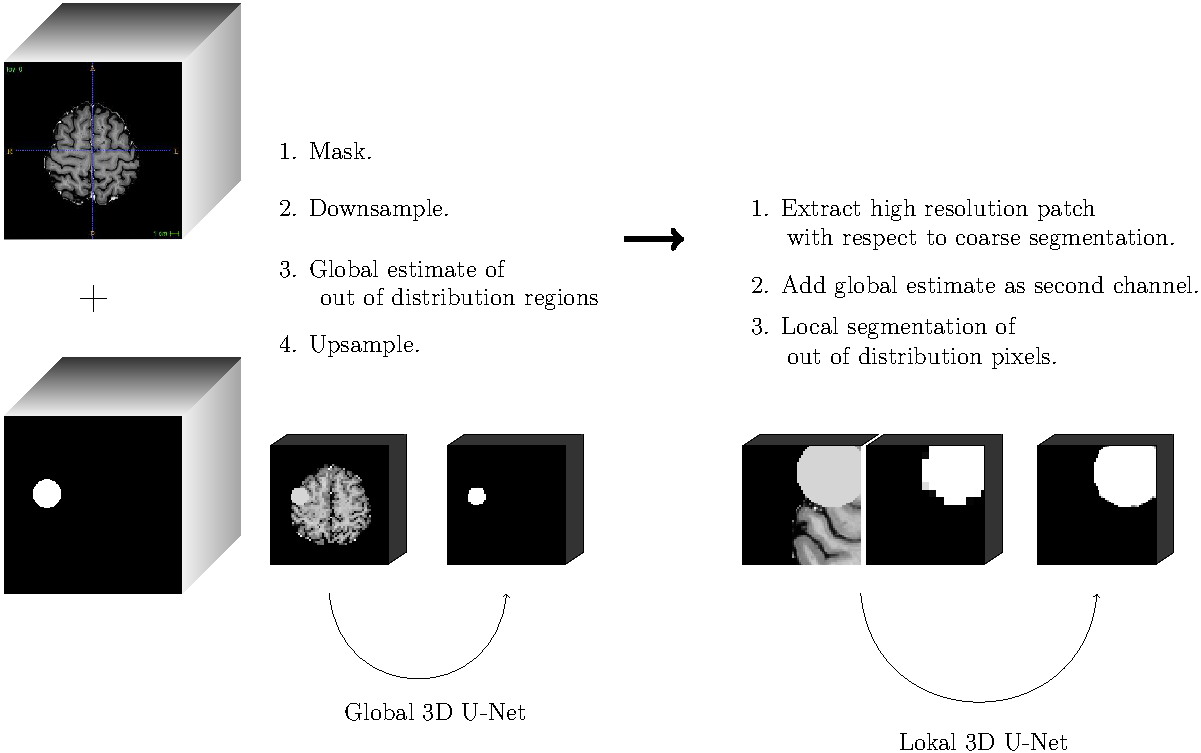
\includegraphics[width=.78\columnwidth]{_figs/method-cropped.pdf}
\end{figure}
\end{frame}


\begin{frame}
\frametitle{Inpainting Masks: Ellipsoids}
\vfill
\begin{minipage}{0.5\textwidth}
An ellipsoid is defind by the equation
\begin{equation*}
E_{abc}^{t} \colon \quad \frac{(x_1-t_1)^2}{a} + \frac{(x_2-t_2)^2}{b} + \frac{(x_2-t_3)^2}{c} \leq 1,
\end{equation*}
where $t = (t_1, t_2, t_3)$. Each single ellipsoid is shown in the Figure. Parameters $a,b,c\in\N$ and $t_i \in \R$ where generated in a random fashion and each ellipse was rotated by a random angle between $0^\circ$ to $90^\circ$ before adding to the full mask. This was iterated until the number of pixels that lie inside an elliposid exceeded a manually set threshold.
\end{minipage}\hfill
\begin{minipage}{0.4\textwidth}
\phantom{abc}\\
\begin{figure}[htb] \centering
         
\includegraphics[height=0.3\textwidth, width=0.3\columnwidth]{_figs/s1_1}
         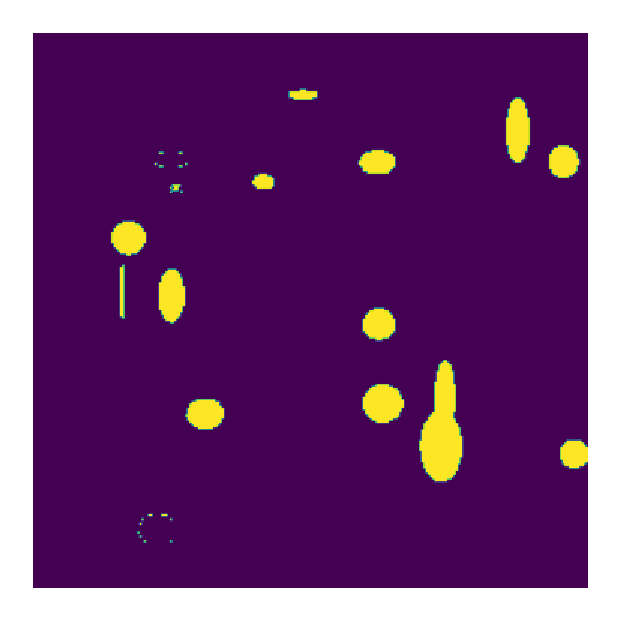
\includegraphics[height=0.3\textwidth, width=0.3\columnwidth]{_figs/s2_1}
         
\includegraphics[height=0.3\textwidth, width=0.3\columnwidth]{_figs/s3_1}\\[0.2em]
         
\includegraphics[height=0.3\textwidth, width=0.3\columnwidth]{_figs/s1_2}
         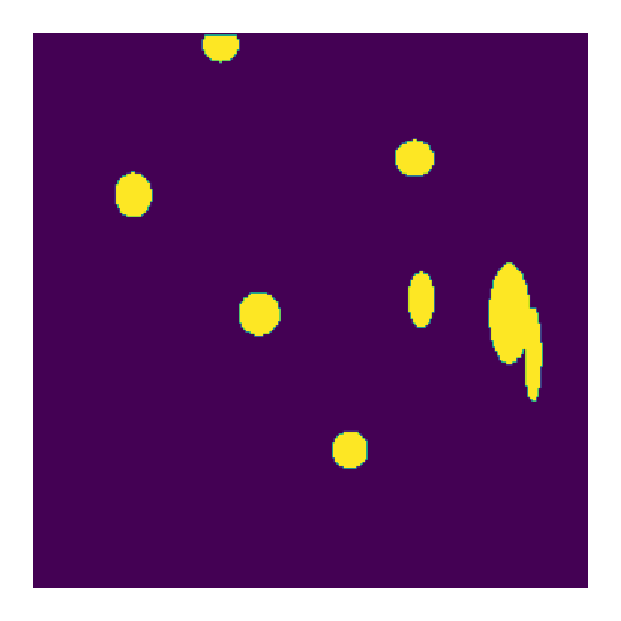
\includegraphics[height=0.3\textwidth, width=0.3\columnwidth]{_figs/s2_2}
         
\includegraphics[height=0.3\textwidth, width=0.3\columnwidth]{_figs/s3_2}
\caption{Visualization of 3D ellipsoid inpainting masks. The projections onto the first, second and third axis, respectively.}
\label{fig:ellipses}
\end{figure}
\end{minipage}
\vfill
\end{frame}



\begin{frame}
\frametitle{Inpainting Masks: $\alpha$-shapes}
\vfill
\begin{minipage}{0.5\textwidth}
First, we randomly select a number of points $x_i, i=1,\ldots N$, that satisfy
\begin{equation*}
\epsilon_1 \leq \norm{x_i - x_j}_2 \leq \epsilon_2,
\end{equation*}
for all $i,j=1,\ldots, N$ and manually chosen $\epsilon_1, \epsilon_2 > 0$.
We then used the Python package $\alpha$-shape (\url{https://pypi.org/project/alphashape/}) to create the $\alpha$-shape of the set $\sparen{x_1, \ldots x_N}$. For $\alpha = 0$, the algorithm producedes the convex hull. Examples on the right where calculated for $\alpha=3$.
\end{minipage}\hfill
\begin{minipage}{0.4\textwidth}
\phantom{abc}\\
\begin{figure}[htb] \centering
         
\includegraphics[height=0.3\textwidth, width=0.3\columnwidth]{_figs/s1_1_concave}
         
\includegraphics[height=0.3\textwidth, width=0.3\columnwidth]{_figs/s2_1_concave}
         
\includegraphics[height=0.3\textwidth, width=0.3\columnwidth]{_figs/s3_1_concave}\\[0.2em]
         
\includegraphics[height=0.3\textwidth, width=0.3\columnwidth]{_figs/s1_2_concave}
         
\includegraphics[height=0.3\textwidth, width=0.3\columnwidth]{_figs/s2_2_concave}
         
\includegraphics[height=0.3\textwidth, width=0.3\columnwidth]{_figs/s3_2_concave}
\caption{Visualization of concave inpainting masks. Two examples are shown in the top and bottom row. The projections onto the first, second and third axis, respectively.}
\label{fig:ellipses}
\end{figure}
\end{minipage}
\vfill
\end{frame}

\begin{frame}{Perturbations}
	\begin{minipage}{.45\columnwidth}
		\begin{center}
			
			\begin{figure}
				\textbf{random intensity}\\[.2em]
				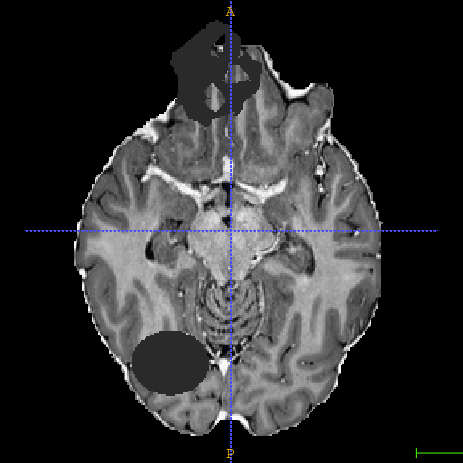
\includegraphics[width=.43\columnwidth]{_figs/int.png}\hfil
				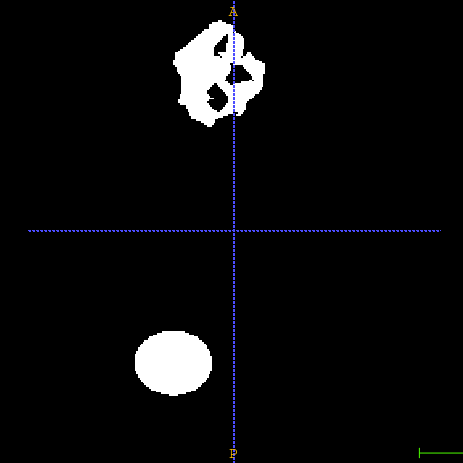
\includegraphics[width=.43\columnwidth]{_figs/intm.png}
			\end{figure}\vspace{1em}
			
		\begin{figure}
			\textbf{Gaussian noise}\\[.2em]
			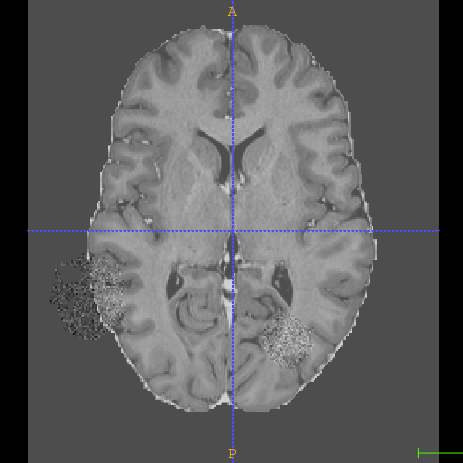
\includegraphics[width=.43\columnwidth]{_figs/gauss.png}\hfil
			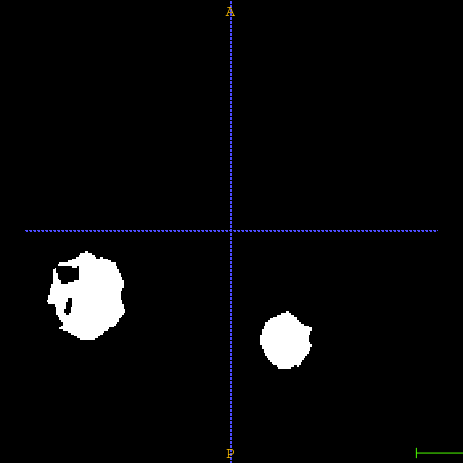
\includegraphics[width=.43\columnwidth]{_figs/gaussm.png}
		\end{figure}
		\end{center}
	\end{minipage}\hfil
\begin{minipage}{.45\columnwidth}
	\begin{center}
		\begin{figure}
			\textbf{scaled intensity}\\[.2em]
			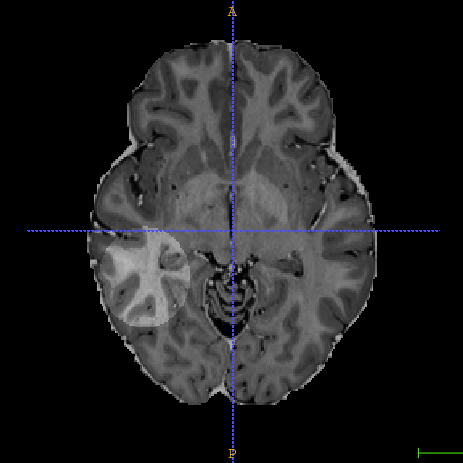
\includegraphics[width=.43\columnwidth]{_figs/scale.png}\hfil
			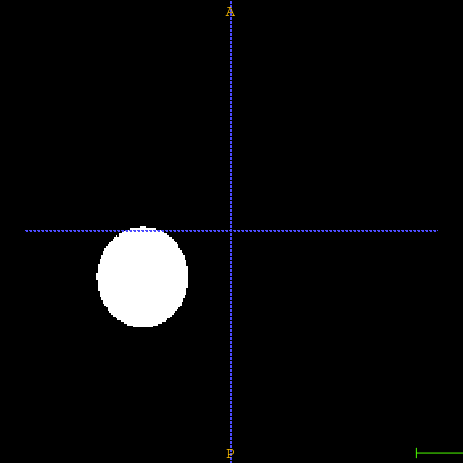
\includegraphics[width=.43\columnwidth]{_figs/scalem.png}
		\end{figure}\vspace{1em}
			
		\begin{figure}
			\textbf{Sobel filter}\\[.2em]
			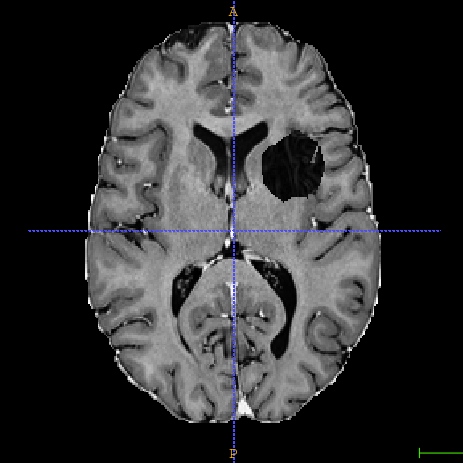
\includegraphics[width=.43\columnwidth]{_figs/sobel.png}\hfil
			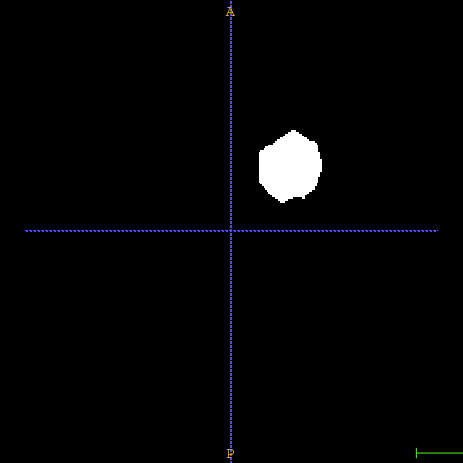
\includegraphics[width=.43\columnwidth]{_figs/sobelm.png}
		\end{figure}
	\end{center}
\end{minipage}
\end{frame}

\begin{frame}{Limitations}
	\begin{itemize}
		\item Sub-sampling yields the issue that some disturbances, such as Gaussian noise, get reduced and are therefore harder to detect.
		\item Since the predictions only get refined in areas where the global prediction has exceeded a threshold of predicted out-of distribution pixels, it is possible that very small objects are overlooked.
		\item The variety of synthetic data is limited and could be insufficient for detecting certain naturally occurring anomalies.
	\end{itemize} \pause \vspace{1.5em}
	
	{\Large\textbf{Possible improvements: }}\pause \vspace{1em}
	\begin{itemize}
		\item Combine different downsampling methods.
		\item Increase the diversity of the synthetic anomalies.
	\end{itemize}
	
\end{frame}


%%%%%%%%%%%%%%%%%%%%%%%%%%%
%% to show a last slide similar to the title slide: information for the last page
\title{Thank you for your attention!}
\subtitle{}
\author{}
\section{Thanks}



\end{document}